\section{Cache Test Week 4}

When running the \texttt{cachetest.c} file, we get a list of times for different chache tests. From this, we will try to distinguish the cache line size, Li size, L2 size and L3 size.

If we analyze them in order, we first look for the cache line size. We suspect the read/write times to go up, as cache misses increase. When the stride length in the cachetest.c succeed our cache line size, more misses will occur, since the next procedure also misses subsequently. This should be clear when trying to allocate a large array, since the look-ups at cache misses will stand out. 

\begin{figure}[h]
    \centering
    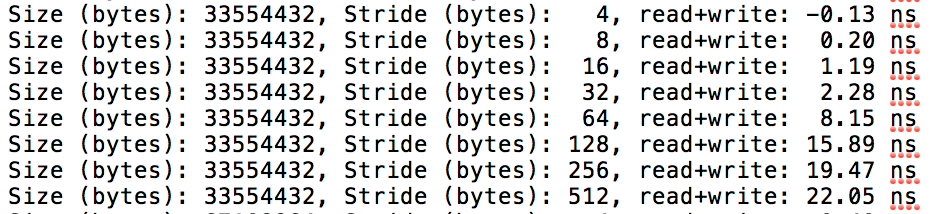
\includegraphics[width=\linewidth]{Week4/fig/CacheBlock.png}
    \caption{Times showing the cache line as the highest relative jump in time.}
    \label{fig:cacheblock}
\end{figure}

In fig \ref{fig:cacheblock} we see the biggest relative jump (\textbf{x}4) when going from a stride length of 32 bytes to 64 bytes. This suggests that our line size is either of theses two sizes, depending on how the line content is chosen when caching. 

Next step is to find the sizes of L1, L2 and L3 cache. If the complete array is stored in cache, the times should not go up no matter the stride length. When the data structure can no longer be contained in the different cache levels, the sizes of these cache levels should then be seen as a sudden spike in time (most significant when stride succeeds the cache line size). The stride lengths are not shown in fig \ref{fig:misses}, but the ordering is not altered compared to fig \ref{fig:cacheblock}.

\begin{figure}[ht]
\centering
    \begin{subfigure}{0.4\textwidth}
    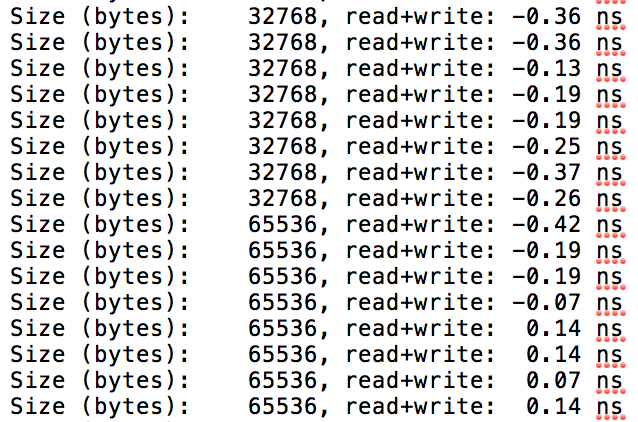
\includegraphics[width=\linewidth]{Week4/fig/L1Miss.png} 
    \caption{ }
    \label{fig:L1}
    \end{subfigure} 
    
    \begin{subfigure}{0.4\textwidth}
    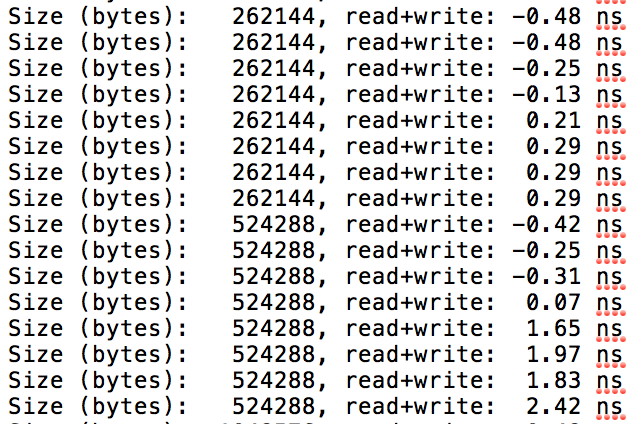
\includegraphics[width=\linewidth]{Week4/fig/L2Miss.png}
    \caption{ }
    \label{fig:L2}
    \end{subfigure}
    
    \begin{subfigure}{0.4\textwidth}
    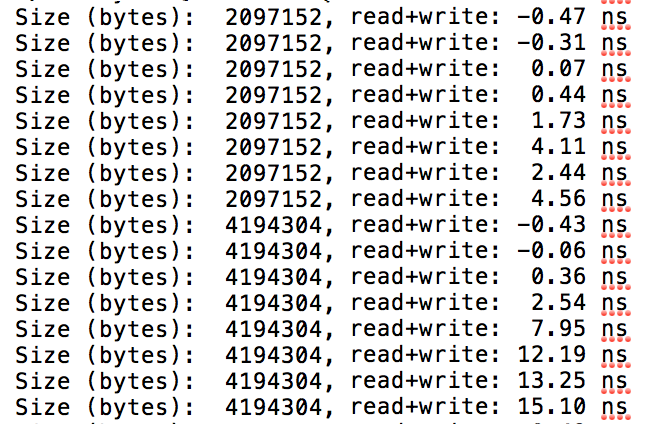
\includegraphics[width=\linewidth]{Week4/fig/L3Miss.png}
    \caption{ }
    \label{fig:L3}
    \end{subfigure}
    
    \caption{Cache misses showing: a) L1 limit, b) L2 limit and c) L3 limit.}
    \label{fig:misses}
\end{figure}

As seen in fig \ref{fig:L1}, the first jump in time is from 32kB to 64kB, suggesting that this system has a L1 cache size of around 32kB. Using the same reasoning fig \ref{fig:L2} and \ref{fig:L3} suggest that the L2 cache size is around 258kB and L3 cache size is around 2MB or 3MB. 

Looking up the computer specifications, we see that indeed the cache line size is 64 bytes, L1 has size 32kB (each of dcache and ichache), L2 has size 258kB and L3 has size 3MB. 

To alter the \texttt{cachetest.c} file for better read/write speeds, we need to make sure, that subsequent operations optimize for reusing cached memory. In the first do-while loop, the two for-loops control how the memory is accessed in the array \texttt{x}. The innermost loop increments the index by the stride length. This means, that every look-up is at a new position. If the two for loops change order, the index is constant for every iteration of the innermost loop. This will minimize cache misses, since two subsequently look-ups of the same memory, is \textit{almost} guaranteed to be cached. Running the program again, we see that all the times are now below 0.4 ns. 

This means, in order to optimize future programs for cache, we need to take the sizes of L1 to L3 cache into consideration when creating data structures. If an array is used, which can be fully stored e.g. in the 32kB L1 dcache, together with the various local variables, memory access would be optimal. If larger data structures are needed, the size of the cache line (in this case 64 bytes) is important, since the subsequent memory accesses' would be contained in the cache line, if the information is contained from the loaded memory block in the cache line. In general cache hits would also be likely when reusing variables, instead of accessing new memory addresses each time (or rather, the the address modulus the number of cache lines $32\text{kB}/64\text{B} = 500$ for L1 if directly mapped). Most operating systems don't use directly mapped cache, but instead a form of set-associative caching. This means, that conflicts in cached memory is less, and the general strategy is; grouping variables, and accessing data with short intervals, optimizing for space and time locality. 

The attached file \texttt{cachetest.c} containes the source code discussed.